% !TeX root = ../main.tex
\chapter{SLAM在地图构建方面的应用}
SLAM全称同时定位与地图构建,在前面我们一直讨论的是定位问题,但这并不表示建图就不重要。一是因为前面的定位、位姿优化等是建图的基础,二是因为人们对建图的要求不同,有的需要简单的稀疏地图,有的需要稠密的地图,大致归纳如下:\par
\begin{enumerate}
	\item 定位:定位是地图的基本功能。在前面的视觉里程计部分,我们讨论了利用局部地图来实现定位;在回环检测部分,我们发现只要有全局描述子信息,机器人的位置信息还能通过回环检测来确定。更进一步,我们还希望地图能够保存下来,分享给其它经过相似场景的机器人,这样我们就能够实现经过一次建模,地图共享。
	\item 导航:导航是指机器人通过视觉或其它传感器信息在地图中进行路径规划,最终到达目的地。稀疏的地图已经不能满足导航的需求,我们需要建立稠密地图。
	\item 避障:避障导航类似需要规划路径避开障碍物,但更注重局部的、动态的障碍物的处理。但仅有稀疏的特征点,我们还很难判断某个特征点是否为障碍物, 所以我们还需要稠密地图。
	\item 重建:重建地图主要用于展示、通讯、增强现实等,这样的地图要求舒服、美观。这种地图也要求是稠密的,而且对它的外观有一些要求,希望能够构建带有纹理的平面。
	\item 交互:交互主要指人与地图之间的互动,这要求机器人对地图有更高层面的认知,这种地图也被称为语义地图。
\end{enumerate}
在这里我们简单介绍一种三维重建的方法:PatchMatch\par
PatchMatch的基本思想是假设图像中相邻的像素区域更可能在同一个平面上。这种算法用近乎随机的方法进行全像素计算得到稠密深度图。PatchMatch算法还设计了一个传播的过程,也就是说如果一个点的深度找的很好,那我们可以做出相邻点的深度和平面和该点差不多的假设。那么即便我们随机初始化深度图,只要有一个找到好,这样好的深度就会扩散开,让所有点受益。
\begin{figure}[H]
	\centering
	\begin{subfigure}[ht]{0.4\textwidth}
		\centering
		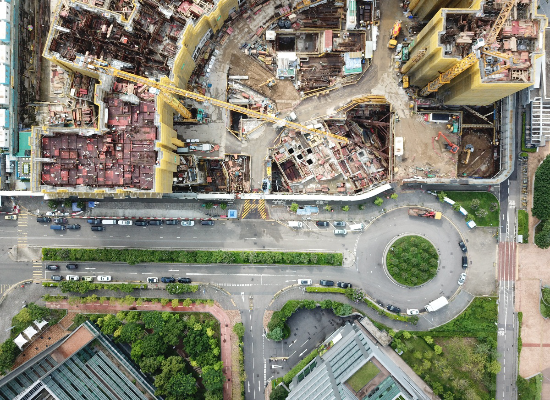
\includegraphics[height=4cm]{fig1_1}
	\end{subfigure}
	\quad
	\begin{subfigure}[ht]{0.4\textwidth}
		\centering
		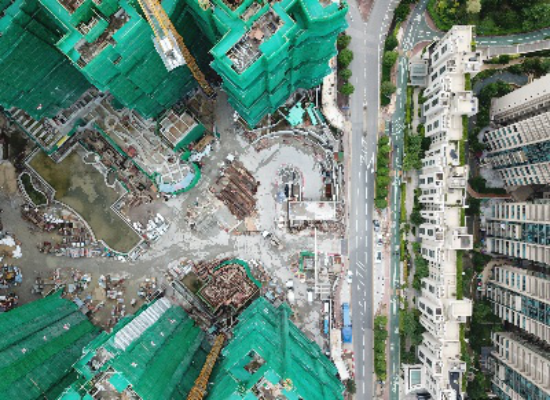
\includegraphics[height=4cm]{fig2_1}
	\end{subfigure}\\
	\begin{subfigure}[ht]{0.4\textwidth}
		\centering
		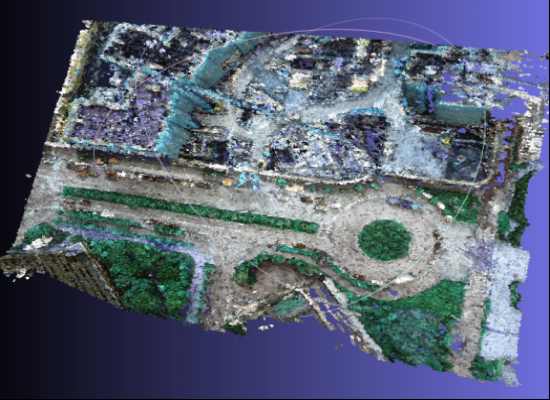
\includegraphics[height=4cm]{re1_1}
	\end{subfigure}
	\quad
	\begin{subfigure}[ht]{0.4\textwidth}
		\centering
		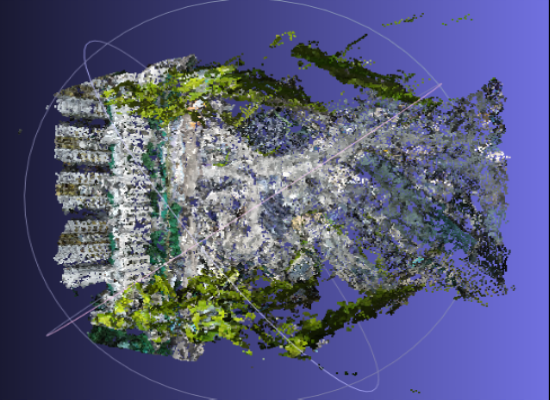
\includegraphics[height=4cm]{re2_1}
	\end{subfigure}
\begin{subfigure}[ht]{0.4\textwidth}
	\centering
	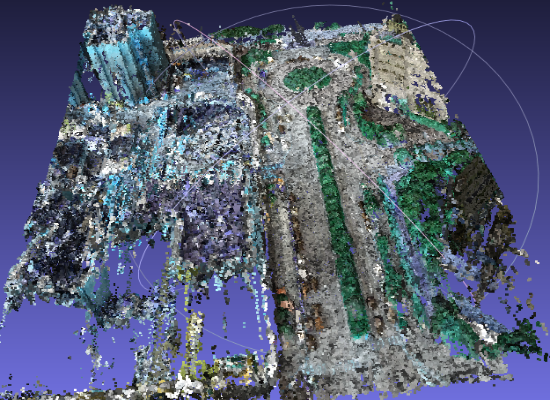
\includegraphics[height=4cm]{re1_2}
	\subcaption{场景a}
\end{subfigure}
\quad
\begin{subfigure}[ht]{0.4\textwidth}
	\centering
	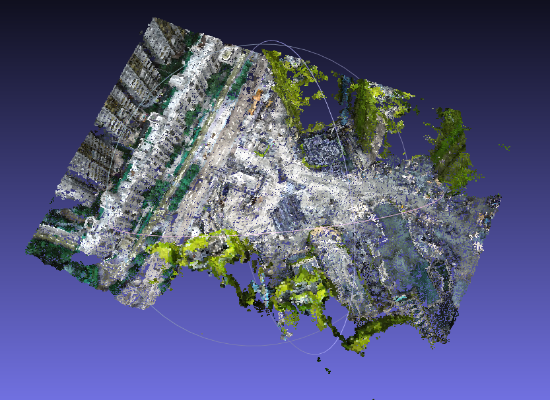
\includegraphics[height=4cm]{re2_2}
	\subcaption{场景b}
\end{subfigure}
	\caption{PatchMatch}
\end{figure}






